%==============================================================================
%  SeMaNa @ IROS 2026 — extended abstract (2–4 pp, refs excluded)
%  Double-blind, non-archival.  IEEE RAS double-column.
%
%  DRAFTING NOTES
%  - Guidance under each (sub)section is in "% POINTS TO HIT:" comments, lifted
%    from docs/WORKSHOP_PAPER_PLAN.md.  Write the prose in YOUR OWN words and
%    delete the comment as you go.
%  - Tables are pre-filled with the final numbers (regen via scripts/agg_*.py).
%  - Figures point at results/paper/_figs/*; copy/symlink into paper/figs/.
%  - Build:  pdflatex main && bibtex main && pdflatex main && pdflatex main
%==============================================================================
\documentclass[conference]{IEEEtran}
\IEEEoverridecommandlockouts

\usepackage{graphicx}
\usepackage{booktabs}
\usepackage{float}      % provides [H] — force a float exactly in place (never dropped)
\usepackage{subcaption}
\usepackage{amsmath,amssymb}
\usepackage{url}
\usepackage{xcolor}
\usepackage[hidelinks]{hyperref}

\graphicspath{{figs/}}

% Relax float placement so the many result floats all place in a float-heavy,
% text-light draft (avoids tail tables/figures being deferred/dropped).
\setcounter{topnumber}{4}
\setcounter{totalnumber}{6}
\renewcommand{\topfraction}{0.95}
\renewcommand{\textfraction}{0.05}
\renewcommand{\floatpagefraction}{0.75}
\renewcommand{\dbltopfraction}{0.95}
\renewcommand{\dblfloatpagefraction}{0.75}

% Drafting helper — remove before submission.
\newcommand{\todo}[1]{\textcolor{red}{[\textbf{TODO:} #1]}}

\begin{document}

%------------------------------------------------------------------------------
% TITLE  (pick one; see plan §Title candidates)
%   A) Making a Shape Generator a Scene Creator: Instance-Forward Asset Mapping
%      for Metric-Semantic Scene Graphs
%   B) Beyond Shape: Placing Single-Image 3D Generations in a Metric Robot
%      Scene Graph
%------------------------------------------------------------------------------
\title{Making a Shape Generator a Scene Creator:\\
Instance-Forward Asset Mapping for Metric-Semantic Scene Graphs}

% DOUBLE-BLIND: keep anonymous.
\author{\IEEEauthorblockN{Anonymous Submission}
\IEEEauthorblockA{SeMaNa @ IROS 2026 --- Paper \#XXX}}

\maketitle

%------------------------------------------------------------------------------
\begin{abstract}
% POINTS TO HIT (write last, ~120 words):
% - Robots in human spaces need object-centric METRIC maps whose nodes are
%   complete, placed 3D objects (sim/manipulation ready), not labeled clusters.
% - Single-image 3D generators (SAM 3D) make excellent SHAPES but do not build
%   a scene: they decide neither what objects exist, nor where, nor how big.
% - We pair an instance-forward multi-view front-end (what exists) with a
%   metric-placement back-end (where/how big) -> asset-centric scene graph of
%   Sim(3)-registered, simulation-ready meshes.
% - Three single-variable results: C1 registration supplies pose SAM 3D can't;
%   C2 generation completes unobserved geometry; C3 net map places metrically
%   where clustering only localizes coarsely. Shown in ProcTHOR sim (real GT
%   meshes) + a deployed Go2 quadruped.
%
% HIGHLIGHT METRICS — weave 2-3 of these into the last sentence(s). Use the
% comparison framing shown; DON'T strip the "vs what" or the guardrails.
%   C1 (sim, ours vs SAM 3D's own placement): 3D-IoU F1 0.40 -> 0.49 (+20%),
%       recall@0.5 0.15 -> 0.22 (+52%), rotation 9.7deg -> 6.8deg.
%   C2 (sim, oracle-placed, the "why generate" number): the generated asset
%       reconstructs UNOBSERVED surface ~2.9x better than the observed cluster
%       at low coverage (0.08 vs 0.23 m); 166/212 objects favor the asset.
%   C3 (real Go2, ours vs independently-run Clio): strict 3D-IoU F1 4-5x higher
%       (0.17 vs 0.04) at comparable open-set recall (class-free 0.75 vs 0.69);
%       scale-fit cuts real scale error, paired per-object median 0.74 -> 0.59
%       (Wilcoxon p<1e-4).
%   PICK: C1's +20%/+52% and C2's 2.9x are the punchiest + safest. If you cite
%   C3, keep "vs an independently-run baseline" and lead scale, not IoU alone.
%   AVOID in the abstract: any blanket "SAM 3D scale is 3x off" (it's regime-
%   dependent) and any centroid-improvement claim on real (selection artifact).
\todo{write abstract last — weave in 2-3 highlight metrics above}
\end{abstract}

%==============================================================================
\section{Introduction}
%==============================================================================
% WRITE THIS SECTION YOURSELF from the topic-sentence bullets below (~3/4 col).
% One paragraph per (P#) bullet is a reasonable target. These are prompts, not
% prose — say each in your own words.
%
% (P1) MOTIVATION — the map robots actually need.
%   - Robots acting in human spaces need object-centric *metric* maps whose
%     nodes are complete, placed 3D objects — usable for simulation and
%     manipulation — not labeled point clusters.
%   - [v1 salvage, optional hook] Humans encode space semantically, not as raw
%     metric grids (place/grid cells); the useful robot map fuses semantics WITH
%     metric detail. (v1 refs [1]-[6] if you want the neuroscience opener.)
%
% (P2) THE TENSION — a spectrum with a gap in the middle.
%   - [v1 "spectrum" device, re-keyed] On one end, scene-level mapping
%     (SLAM/NeRF/Gaussian-splat, Kimera/Hydra) captures global layout but no
%     object-level geometry; on the other, single-image 3D generators (SAM 3D)
%     now make excellent object *shapes*.
%   - THE SHARPENED TURN (this is the new thesis, NOT v1's "best of both
%     worlds"): a shape generator is not a scene builder — it decides neither
%     what objects exist, nor where they are in the world, nor how big.
%
% (P3) OUR MOVE — shape generator -> scene creator.
%   - Pair an instance-forward multi-view front-end (decides WHAT exists) with a
%     metric-placement back-end (decides WHERE / HOW BIG) -> an asset-centric
%     scene graph whose nodes are Sim(3)-registered, simulation-ready meshes.
%   - HONESTY GUARDRAIL: the front-end is infrastructure, same family as
%     ConceptGraphs/HOV-SG — NOT claimed as novel. The differentiator is the
%     node PAYLOAD (a placed, simulatable mesh vs a labeled point cluster).
%   - Disambiguation (do on first mention): SAM 3 = 2D detect/seg/track;
%     SAM 3D = the single-image shape generator we build on.
%
% (P4) CONTRIBUTIONS — three single-variable results (forward-ref C1/C2/C3):
%   - C1: registration supplies the metric pose/scale SAM 3D cannot.
%   - C2: generation completes the geometry the robot never observed.
%   - C3: the net map places objects metrically where the clustering
%         scene-graph line only localizes them coarsely.
%   - Shown in ProcTHOR sim (real GT meshes -> shape fidelity) AND on a deployed
%     Go2 quadruped (metric placement). Close on the deliverable: an
%     asset-centric USD map, not a labeled cluster set.

%==============================================================================
\section{Related Work}
%==============================================================================
% DRAFT — rewrite in your own voice; may need trimming to ~1/2 col for the
% extended-abstract budget. Honesty guardrails are baked in: (i) do NOT claim a
% novel/superior front-end, (ii) the differentiator is the NODE PAYLOAD, (iii)
% disambiguate SAM 3 from SAM 3D.

\subsection{Object-Centric Metric--Semantic Scene Graphs}
Our system belongs to the now-established family of object-centric
metric--semantic maps built online from a moving open-vocabulary sensor.
Hydra~\cite{hydra} and Khronos~\cite{khronos} construct a global labelled 3D map
and derive object nodes by clustering it, whereas ConceptGraphs~\cite{conceptgraphs},
HOV-SG~\cite{hovsg}, and Clio~\cite{clio} are instance-forward: they lift
per-frame open-vocabulary masks into 3D and fuse them into per-object point
clusters. SuperMap~\cite{supermap} sharpens this line with 3D-anchored
tracking-by-detection that it shows outperforms point-feature clustering for
online instance mapping. Our front-end is deliberately a member of this
instance-forward family --- architecturally closest to
ConceptGraphs/HOV-SG --- and we make \emph{no} claim that it is novel. What
differs is the \emph{node payload}. Where these systems represent an object as a
labelled point cluster or bounding box, each node in our map is a generated,
$\mathrm{Sim}(3)$-registered, watertight mesh with a well-posed metric box: a
simulation-ready asset. This is the row the clustering line cannot fill, and it
is the contribution we claim; we evaluate against it directly by running
Clio~\cite{clio} on our robot data under identical ground truth and metrics
(Sec.~\ref{sec:experiments}).

\subsection{Single-Image 3D Generation and Scene Completion}
The node payload comes from single-image 3D generation. SAM 3D~\cite{sam3d}
turns a single masked crop into a high-quality object mesh, and shape/scene
completion methods such as SceneComplete~\cite{scenecomplete} and
MetaScenes~\cite{metascenes} reconstruct or curate object arrangements from
imagery. These methods produce excellent geometry, but under conditions a robot
does not enjoy --- a clean, well-framed crop, a curated scene, or a human in the
loop --- and they treat metric placement as given or hand-authored. A
single-image generator in particular decides neither what objects are present,
nor where they sit in the world, nor how big they are: its predicted translation
and scale are in normalized camera coordinates and unreliable on real
imagery. We therefore use SAM 3D for \emph{shape only} and supply the rest
autonomously --- an instance-forward front-end decides what exists from partial
egocentric views, and a metric back-end registers each generated shape into the
scene at the observed depth --- turning a shape generator into a scene creator.

% Disambiguation — keep it; reviewers conflate the two names.
\subsection{A Note on Naming}
To avoid a common conflation: SAM 3~\cite{sam3} is a 2D model for
open-vocabulary detection, segmentation, and tracking, whereas
SAM 3D~\cite{sam3d} --- the model we build on --- is a single-image 3D shape
generator. The two are distinct despite the shared name, and neither is Yang
\emph{et al.}'s SegmentAnything3D.

%==============================================================================
\section{Method}
%==============================================================================
% DRAFT — rewrite in your own voice. Notation reused from v1; front-end kept
% deliberately humble (it is infrastructure, not a claimed contribution).
\begin{figure}[htbp]
  \centering
  % Fig 1 — pipeline teaser: robot -> tracks -> registered assets -> USD in Isaac Sim
  % \includegraphics[width=\linewidth]{fig1_pipeline}
  \fbox{\parbox{0.95\linewidth}{\centering\vspace{2.5em}Fig.~1 pipeline teaser\\(robot $\to$ tracks $\to$ registered assets $\to$ USD)\vspace{2.5em}}}
  \caption{\todo{pipeline teaser caption}}
  \label{fig:pipeline}
\end{figure}

We assume the robot has an estimate of its pose $s_t \in \mathrm{SE}(3)$ at each
time $t$ (from onboard localization or odometry) and observes an RGB-D stream
$y_t = (y_t^{\text{rgb}}, y_t^{\text{depth}})$ from a stereo camera with known
intrinsics. Our goal is an object-centric scene $\xi_t = \{o_k\}$ in which every
node $o_k$ is a 3D mesh placed by a similarity transform $x_k \in
\mathrm{Sim}(3)$ --- a pose \emph{and} a metric scale --- rather than a labelled
point cluster. The pipeline (Fig.~\ref{fig:pipeline}) has three stages: an
instance-forward front-end that decides \emph{what objects exist}
(Sec.~\ref{sec:frontend}), a single-image generator that supplies each node's
\emph{shape} (Sec.~\ref{sec:node}), and a metric back-end that decides
\emph{where and how big} each object is (Sec.~\ref{sec:backend}). The first
stage is standard machinery, included because it feeds generation and placement;
our contribution is the node payload and how it is placed, not the front-end.

\subsection{Instance-Forward Front-End}
\label{sec:frontend}
Each frame is passed to YOLOE~\cite{yoloe}, an open-vocabulary detector and
segmenter that we prompt with the scene's class vocabulary to obtain a set of
2D object masks with labels and per-frame confidences. Each detection is
back-projected using its masked depth and, following the tracking-by-detection
line~\cite{conceptgraphs}, associated across frames into an \emph{object track}
$k$ by Hungarian matching on a cost that combines the overlap between the
detection mask and the track's reprojected cloud, appearance-embedding
similarity, and 3D-centroid proximity. A track accumulates a
voxel-downsampled, multi-view \emph{fused point cloud} $P_k$ and retains the set
of frames in which it was observed; a re-identification and late-merge step
folds fragmented tracks that belong to the same physical object. A track
\emph{matures} once it has been observed in at least three frames, which
suppresses spurious single-frame detections. Finally, for each mature track we
select a single \emph{best view} --- the least-occluded, most-centred frame ---
whose full image and mask are the input to generation. This front-end is
architecturally standard (cf.~\cite{conceptgraphs,hovsg}); we make no novelty
claim for it.

\subsection{Generative Node --- SAM 3D, Shape Only}
\label{sec:node}
Each mature track's best view is sent once to SAM 3D~\cite{sam3d}, a single-image
generative model that reconstructs a watertight object mesh. We pass the
\emph{full frame} together with the object mask rather than a tight crop, which
roughly halves downstream placement error by preserving scene context. From
SAM 3D's output we keep \emph{only the mesh}. SAM 3D also predicts an object
pose, but it does so by flow matching in normalized camera
coordinates~\cite{flowmatching}, which is unreliable on real imagery; we therefore
\emph{discard its predicted translation} entirely, use its predicted rotation
only to seed registration, and treat its scale as an initial estimate to be
refined against sensor depth. This is the crux of the design: SAM 3D is a shape
prior, not a localizer. Because generation is invoked once per object from a
single best view (SAM 3D takes on the order of 20--30\,s per object), the
multi-view front-end earns its cost by choosing that view well and by supplying
the depth the back-end registers against.

\subsection{Metric-Placement Back-End}
\label{sec:backend}
The back-end fixes the object's metric size and pose in two steps. We first set
scale by a \emph{reprojection fit}. The two frontal (in-plane) extents of the
object are read directly from the clean 2D detection mask: we run PCA on the
mask pixels to obtain two principal pixel spans and convert each to metric units
by
\begin{equation}
  e = \frac{s_{\text{px}}\; \tilde{d}}{f},
  \label{eq:reproj}
\end{equation}
where $s_{\text{px}}$ is the pixel span, $\tilde{d}$ is the robust (median)
masked depth, and $f$ the focal length. The third, along-ray axis is never
observed by a single view, so it inherits SAM 3D's shape aspect: matching the
sorted mesh OBB extents $m_1\!\ge\!m_2\!\ge\!m_3$ to the two in-plane fits
$e_1,e_2$, the unobserved extent is
\begin{equation}
  e_3 = m_3\cdot\tfrac{1}{2}\!\left(\frac{e_1}{m_1}+\frac{e_2}{m_2}\right),
  \label{eq:third}
\end{equation}
and an anisotropic scaling of the mesh about its OBB centre applies
$(e_1,e_2,e_3)$. We read scale from the mask
rather than from the depth cloud deliberately: the mask agrees with the object
silhouette (IoU $\approx 0.96$) where the raw depth cloud is edge-contaminated
and one-sided, so its object-boundary extent is far more reliable. We then
refine \emph{pose} with point-to-point ICP~\cite{icp},
\begin{equation}
  T^\star=\arg\min_{T\in\mathrm{SE}(3)}\sum_i \big\lVert T x_i - y_{\pi(i)}\big\rVert_2^2,
  \label{eq:icp}
\end{equation}
over mesh surface points $\{x_i\}$ and their nearest points $\{y_{\pi(i)}\}$ in
the track's fused cloud $P_k$, initialized at the SAM 3D seed pose $T_0$
(predicted rotation placed at the observed depth) and reverting to $T_0$ when
the inlier fitness falls below a threshold. ICP carries no scale degree of
freedom, so it only nudges the object off $T_0$. Optionally the scale and pose
steps alternate to convergence.

A lightweight \emph{precision gate} then demotes a mature track unless it clears
a minimum number of observations and a minimum mean detection confidence,
pruning short-lived false-positive tracks. The resulting object-centric scene
graph is serialized to USD/GLB for use in simulation.

This split follows a single design principle. Scale depends on the object's
\emph{true boundary} --- an extremum statistic that a few stray depth points
inflate and that a one-sided view gets wrong regardless of noise --- so we read
it from the clean RGB mask plus the shape prior. Pose depends on the
\emph{bulk surface} --- a summed nearest-neighbour average dominated by the
object body --- so rigid ICP on the same imperfect cloud is robust, provided it
is denied a scale degree of freedom. Sec.~\ref{sec:experiments} shows that
reading extent from the depth-cloud bounding box instead craters accuracy, while
ICP on that same cloud remains fine.

%==============================================================================
\section{Experiments}
\label{sec:experiments}
%==============================================================================
% FRAMING SENTENCE (hit first): two regimes, single-variable CONTROLLED
% comparisons rather than confounded system-vs-system bake-offs —
%   ProcTHOR sim (real GT asset meshes -> shape fidelity) and a real Go2 in four
%   scenes (cuboid GT -> metric placement).

\subsection{Setup and Metrics}
\label{sec:metrics}
% NOTE: full metric definitions + per-table configs are in the Appendix
% (App~\ref{app:metrics} / App~\ref{app:config}). CHECK THE CFP FIRST: workshop
% page limits usually COUNT appendix pages, so this may be a "what's essential"
% decision, not free space — see chat.
We evaluate in two regimes. In simulation we use ten held-out ProcTHOR scenes
whose ground-truth objects are real asset meshes, letting us score shape
fidelity directly; on hardware we use four scenes captured by a Go2 quadruped
with a RealSense camera, where ground truth is hand-labelled oriented boxes and
the question is metric placement. The same detector (YOLOE prompted with the
scene vocabulary) and depth feed drive every configuration, so each comparison
varies a single factor.

Every comparison is single-variable: the front-end (YOLOE prompted with the
scene vocabulary), tracker, depth, and metric code are held fixed while one
factor --- node payload, registration mode, or scale source --- changes. The
SAM 3D meshes are generated once and re-scored across registration modes, so
placement comparisons are exact, and our external baseline (Clio~\cite{clio}) is
run by us under the same ground truth and metrics. Appendix~\ref{app:config}
details the per-table configurations, datasets, and the paired-object scale test
used on the small real-scene matched sets.

We report metrics at two strictness levels, since a labelled-cluster baseline
and an asset map can tie on \emph{whether} an object was found while differing on
\emph{how well} it is placed and sized. Predictions are matched to ground truth
by Hungarian assignment on 3D oriented-box IoU above a threshold; with
$\mathrm{TP}$ matched pairs the headline \emph{IoU-F1} is
\begin{equation}
  \mathrm{F1}=\frac{2\,\mathrm{P}\,\mathrm{R}}{\mathrm{P}+\mathrm{R}},\quad
  \mathrm{P}=\frac{\mathrm{TP}}{|\{p_i\}|},\quad
  \mathrm{R}=\frac{\mathrm{TP}}{|\{g_j\}|},
\end{equation}
at IoU $\ge 0.25$ ($\text{recall@}0.5$ repeats it at $0.5$). On matched pairs we
report centroid error, orientation error, and the \emph{scale error}
$e_{\text{scale}}=\max_a|\hat{s}_a/s_a-1|$ --- the largest per-axis relative
extent error, our real-robot lead metric --- with Scan2CAD accuracy
($20\,\text{cm}/20^\circ/20\%$). As a \emph{loose} counterpart, robust to exact
box geometry, we match on top-down centroid within $1\,\text{m}$ and report cd-F1
and class-free recall (any prediction near a ground-truth object, regardless of
label), where baselines are competitive. Full definitions of these and the
surface metrics (scene Chamfer, footprint IoU) are in
Appendix~\ref{app:metrics}.

For the shape-completion study (C2) we isolate generation from placement: under
an oracle pose we measure, per object, the observed coverage $c$ against the
fused observed cloud $O$ and the reconstruction of the \emph{unobserved} surface
$U=\{p\in G_o: d(p,O)>\tau\}$ ($\tau=5\,\text{cm}$),
\begin{equation}
  c=\frac{1}{|G_o|}\!\sum_{p\in G_o}\!\mathbf{1}[d(p,O)\le\tau],\qquad
  r(X)=\frac{1}{|U|}\!\sum_{p\in U}\min_{q\in X}\lVert p-q\rVert,
  \label{eq:unobs}
\end{equation}
comparing the generated asset ($X{=}$mesh) against the observed cluster
($X{=}O$) as coverage $c$ varies.

\subsection{C1 --- SAM 3D Is a Shape Prior, Not a Localizer}
% POINTS TO HIT:
% - Sim (val-10): placing by SAM 3D's OWN predicted pose (layout) vs +ICP:
%   IoU-F1 0.404->0.485 (+20%), recall@0.5 0.147->0.224 (+52%), rot ~9.7->6.8.
% - Real (Go2): reprojection scale-fit cuts scale error on real depth —
%   hallway 0.375->0.240.
% - REGIME-DEPENDENT SCALE (do NOT claim a blanket "3x off"): measured aggregate
%   scale error ~27% sim (icp) vs ~37% real (layout). SAM 3D scale reliable
%   in-distribution, degrades OOD -> why scale-fit is ~neutral on sim (icp wins)
%   but helps on real. The "~3x" is upstream worst-case/worst-axis, not ours.

\begin{table}[H]
  \centering
  \caption{Sim, node-payload $\times$ registration (ProcTHOR val-10). Same
  front-end/tracks/depth/metrics; one factor varied.}
  \label{tab:sim}
  \setlength{\tabcolsep}{3pt}
  \footnotesize
  \begin{tabular}{lccccc}
    \toprule
    config & IoU-F1 & rec@.5 & S2C & cent(m) & scale\_err \\
    \midrule
    asset: layout (SAM3D-native)   & 0.40 & 0.15 & 0.08 & 0.09 & 0.32 \\
    asset: \textbf{+ICP (ours)}    & \textbf{0.49} & \textbf{0.22} & 0.09 & 0.07 & 0.32 \\
    asset: +scale+ICP (ours)       & 0.45 & 0.19 & 0.04 & 0.07 & 0.34 \\
    cluster (baseline)             & 0.41 & 0.23 & 0.12 & 0.05 & 0.31 \\
    \bottomrule
  \end{tabular}
\end{table}

% C1 qualitative panel (chair) AND the fig_c1_sim bar chart both dropped: the bar
% just replotted Table~\ref{tab:sim}, and space is tight -- the table carries C1.

\todo{C1 prose (ref Table~\ref{tab:sim})}

\subsection{C2 --- Generation Completes the Unobserved Geometry}
% POINTS TO HIT (the "why generate" — this is the headline result):
% - Sim shape-completion (val-10, 212 objects, ORACLE-placed to isolate shape):
%   generated asset reconstructs the UNOBSERVED surface 2.87x better than the
%   observed cluster at low coverage (0.081 vs 0.232 m, 68/69 objs), collapsing
%   to a tie where well-seen (18% unseen). 166/212 objects favor the asset.
% - Value concentrates in the PARTIAL-VIEW regime real robots live in — NOT a
%   slight average gain.
% - Honest pairing: end-to-end this needs enough observation to register
%   (placement is coverage-limited); oracle placement isolates that the shape
%   prior CARRIES the unseen geometry. Plus: deliverable metrics can't score a
%   watertight, canonically-oriented mesh vs a cluster.

\begin{figure}[htbp]
  \centering
  % built by scripts/figs/fig_completion.py (edit knobs there)
  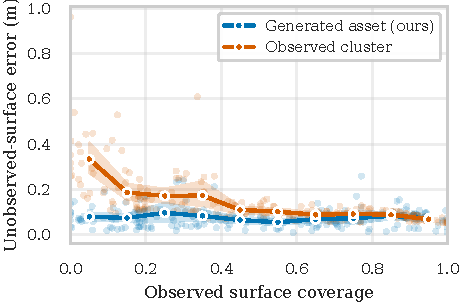
\includegraphics[width=\linewidth]{fig_completion.pdf}\\[3pt]
  % dense, title-less panels from render_completion_panel.py --separate (s200 t26)
  \begin{subfigure}{0.32\linewidth}\centering
    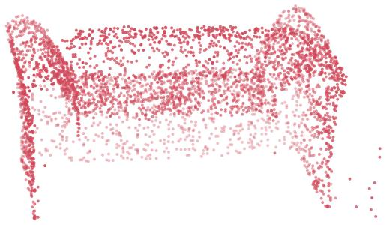
\includegraphics[width=\linewidth]{completion_panel_s200_t26_a}
    \caption{observed}\label{fig:panel_a}
  \end{subfigure}\hfill
  \begin{subfigure}{0.32\linewidth}\centering
    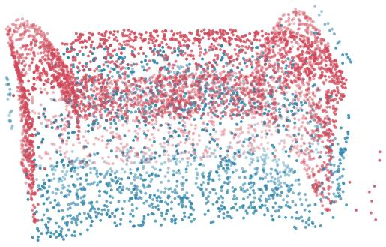
\includegraphics[width=\linewidth]{completion_panel_s200_t26_b}
    \caption{seen + generated}\label{fig:panel_b}
  \end{subfigure}\hfill
  \begin{subfigure}{0.32\linewidth}\centering
    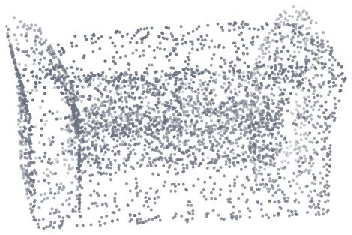
\includegraphics[width=\linewidth]{completion_panel_s200_t26_c}
    \caption{ground truth}\label{fig:panel_c}
  \end{subfigure}
  \caption{\todo{why-generate: (top) unobserved-surface error vs observed
  coverage --- the generated asset (blue) stays flat while the observed cluster
  (orange) degrades sharply as coverage drops (212 objects, val-10); (bottom)
  armchair at 44\% coverage --- red = observed points, blue = generated surface
  filling the unseen base --- vs GT.}}
  \label{fig:completion}
\end{figure}

\todo{C2 prose (ref Fig~\ref{fig:completion}; the metric is $r(X)$, Eq~\ref{eq:unobs}; lead: 0.081 vs 0.232 m, 166/212 favor asset)}

\subsection{C3 --- Metric Placement vs a Clustering Scene-Graph Line}
% POINTS TO HIT:
% - Real (Go2, 4 scenes) vs Clio (run by us, same GT+metrics): on LOOSE open-set
%   recall the two TIE (cd-F1@1m 0.63 vs 0.54; class-free 0.75 vs 0.69 — objects
%   get found); on STRICT metric placement v2 pulls clearly ahead — IoU-F1
%   0.174 vs 0.039 (4-5x), scale-err 0.35 vs 0.55.
% - Contribution ablation (v2-internal; layout -> +icp -> +scale-fit -> +gate):
%   attribute SCALE ACCURACY to scale-fit, PRECISION to the gate.
%
% HONESTY (critical — see plan §Honest read):
% - Scale-fit's real win is SCALE, proven by a PAIRED per-object test (61 objs):
%   median 0.739 -> 0.592, 38/61 objects, Wilcoxon p = 9.5e-5. LEAD THE REAL
%   CLAIM ON THIS, not IoU-F1.
% - Do NOT claim centroid improvement (paired: unchanged, p=0.33 — the aggregate
%   was a matched-set selection artifact).
% - IoU-F1 on real is noise-dominated (TP 1-6/scene); floored by ~0.5m centroid
%   scatter from the uncalibrated (orthogonal, one-time-fixable) extrinsic.
% - ICP hurts rotation on real (small-matched-set artifact).
% - The v2-vs-Clio IoU gap is PIPELINE-level (even layout 0.172 >> Clio 0.039);
%   scale-fit's specific contribution is scale accuracy, not that gap.

% Combined real-robot table (external baseline Clio + our registration progression),
% from real_registration_ablation.csv (agg_real.py) + score_clio_baseline.py.
% NOTE the honest read: at +gate ("v2") loose recall drops (cd-F1 0.50 < Clio 0.54);
% it is +scale+ICP (no gate, cd-F1 0.63) that matches/beats Clio on loose recall.
% Lead the SCALE claim on the paired test (Fig.~\ref{fig:c3paired}), not IoU-F1 (noisy,
% TP 1-6/scene). Clio has no comparable rotation -> "---".
\begin{table}[H]
  \centering
  \caption{Real robot (Go2, 4-scene mean): external baseline Clio vs our
  registration progression (\texttt{layout} = SAM 3D-native placement). On
  \emph{loose} open-set recall, +scale+ICP (cd-F1 0.63) matches/beats Clio (0.54)
  --- objects are found --- while the precision gate trades loose recall (0.50)
  for precision. On \emph{strict} placement ours leads throughout (IoU-F1 up to
  0.19 vs 0.04; scale 0.35 vs 0.55). Per-scene TP is small (1--6), so IoU-F1 is
  noisy --- the scale claim is the paired test (Fig.~\ref{fig:c3paired}).}
  \label{tab:real}
  \setlength{\tabcolsep}{4pt}
  \footnotesize
  \begin{tabular}{lcccccc}
    \toprule
    method / reg & IoU-F1 & cent(m) & scale\_err & rot$^\circ$ & cdF1@1m & cf@1m \\
    \midrule
    Clio (indep.)             & 0.04 & 0.32 & 0.55 & --- & 0.54 & 0.69 \\
    \midrule
    ours: layout              & 0.17 & 0.22 & 0.50 & 10.8 & \textbf{0.68} & \textbf{0.76} \\
    ours: +ICP                & \textbf{0.19} & 0.22 & 0.49 & 16.4 & \textbf{0.68} & \textbf{0.76} \\
    ours: +scale+ICP          & 0.14 & \textbf{0.19} & \textbf{0.35} & 17.3 & 0.63 & 0.75 \\
    ours: +gate (v2)          & 0.17 & 0.20 & \textbf{0.35} & 16.6 & 0.50 & 0.61 \\
    \bottomrule
  \end{tabular}
\end{table}

% C3 LEAD FIGURE — the paired per-object scale test (not in any table).
% Built by scripts/figs/fig_c3_real.py.
\begin{figure}[htbp]
  \centering
  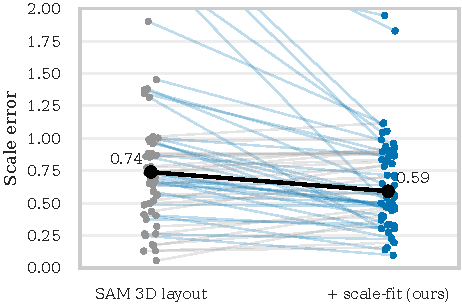
\includegraphics[width=\linewidth]{fig_c3_real.pdf}
  \caption{\todo{C3 lead: paired per-object scale error on the 61 real objects
  matched under both SAM 3D layout and our scale-fit; each line is one object,
  black = medians ($0.74\!\rightarrow\!0.59$; better in 38/61, Wilcoxon
  $p<10^{-4}$).}}
  \label{fig:c3paired}
\end{figure}

\todo{C3 prose (ref Table~\ref{tab:real}, Fig~\ref{fig:c3paired}; LEAD on the paired scale test / Fig~\ref{fig:c3paired})}

\subsection{Why Read Scale off the RGB Mask, Not the Depth Cloud}
% POINTS TO HIT (scale-source ablation, s200 val — supports the design principle):
% - depth-cloud OBB extent CRATERS (fused: scale_err 0.69) — a few edge-bleed
%   points inflate the box; denoising (fused_robust) only partially recovers
%   because the cloud is a one-sided partial view.
% - reading frontal extent from the CLEAN 2D mask (reproj) recovers it.
% - ICP still fine on the same noisy cloud: extent is a max/extremum stat
%   (outlier-fragile); rigid ICP is a bulk/average fit (outlier-tolerant, no
%   scale DOF). -> the design principle from Method.
% (Optional table — include if space allows.)

\begin{table}[H]
  \centering
  \caption{Scale-source ablation (s200 val): read extent from the RGB mask,
  not the depth-cloud OBB.}
  \label{tab:scale_source}
  \setlength{\tabcolsep}{6pt}
  \footnotesize
  \begin{tabular}{lccc}
    \toprule
    scale source & IoU-F1 & scale\_err & Chamfer \\
    \midrule
    fused (raw depth OBB extent)        & 0.16 & 0.69 & 0.25 \\
    fused\_robust (SOR+DBSCAN denoised) & 0.38 & 0.51 & 0.13 \\
    \textbf{reproj (mask span, ours)}   & \textbf{0.51} & 0.32 & 0.09 \\
    icp only (SAM 3D native scale)      & 0.55 & 0.27 & 0.10 \\
    \bottomrule
  \end{tabular}
\end{table}

\todo{scale-source prose (ref Table~\ref{tab:scale_source}) — optional if tight on space}

\subsection{The Front-End Is the Bottleneck}
\label{sec:frontend-bottleneck}
% Reframed to unify the front-end-quality axis: WEAK (YOLOE) -> STRONG (SAM 3,
% App~\ref{app:detector}) -> PERFECT (oracle). Tables kept separate by stride
% (ceiling = val-10 stride 1; SAM 3 sweep = s200 stride 10) -- do NOT merge.
% val-10 means (oracle campaign; regen scripts/agg_oracle.py -> oracle_val10_mean.csv;
% detector rows = Table 1 asset_* val-10 means). Stride 1 both -> no stride confound.
% KEY READS for prose (three, building the axis):
% (1) DETECTION gap: YOLOE+icp 0.49 vs oracle+icp 0.74 (cd-F1 0.71->0.95) -> the
%     front-end, not the back-end, is the bottleneck.
% (2) BACK-END still needed even with PERFECT masks: oracle layout (SAM3D-native,
%     no registration) 0.62 -> oracle +icp 0.74 (+0.12 IoU-F1, rec@.5 0.26->0.33) ->
%     registration is not just cleaning detection noise (reinforces C1). Then
%     scale-fit on clean masks sharpens size (scale 0.29->0.13, S2C 0.12->0.33).
% (3) A STRONGER REAL DETECTOR DOESN'T CLOSE IT (the SAM 3 tie-in, App~\ref{app:detector}):
%     SAM 3 raises open-set recall but not strict placement (it over-detects) and
%     costs ~55x the detector compute -> it is PERFECT MASKS, not a bigger detector,
%     that the ceiling needs. This is the "strong" middle point of the axis.

% Matched-viewpoint scene comparison (shared camera via render_scene --center/--eye;
% RGB from render_thor_rgb.py). SAM3D assets carry per-vertex colour; GT meshes are
% grey geometry. Full-width float; the qualitative companion to Table~\ref{tab:oracle}.
\begin{figure*}[tp]
  \centering
  \begin{subfigure}{0.24\textwidth}\centering
    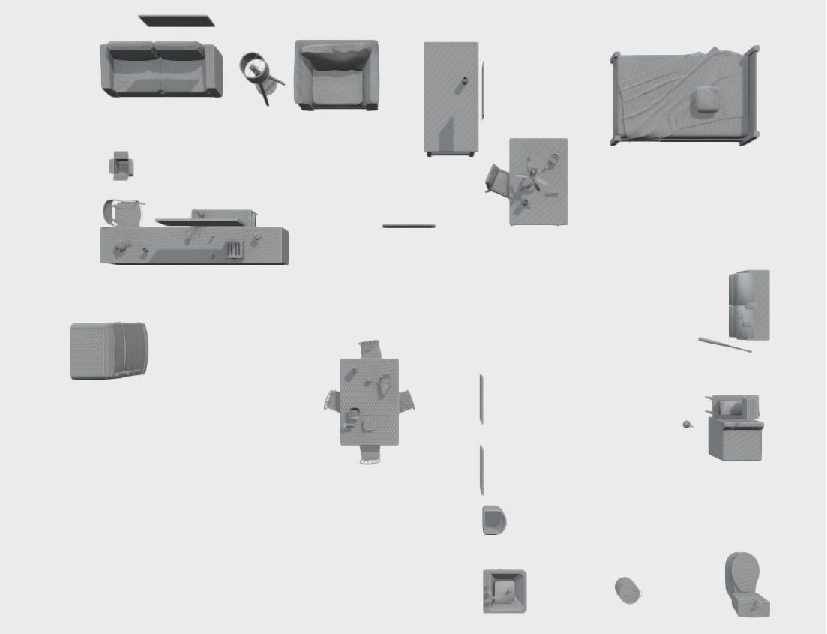
\includegraphics[width=\linewidth]{scene_s200_gt_top.pdf}\caption{GT meshes}\label{fig:scene_gt}
  \end{subfigure}\hfill
  \begin{subfigure}{0.24\textwidth}\centering
    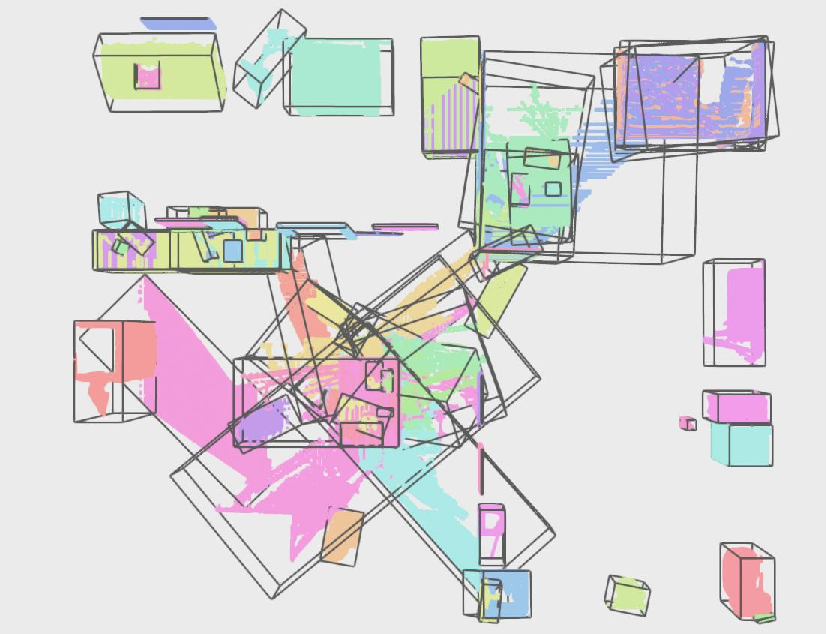
\includegraphics[width=\linewidth]{scene_s200_cluster_top.pdf}\caption{cluster baseline}\label{fig:scene_cluster}
  \end{subfigure}\hfill
  \begin{subfigure}{0.24\textwidth}\centering
    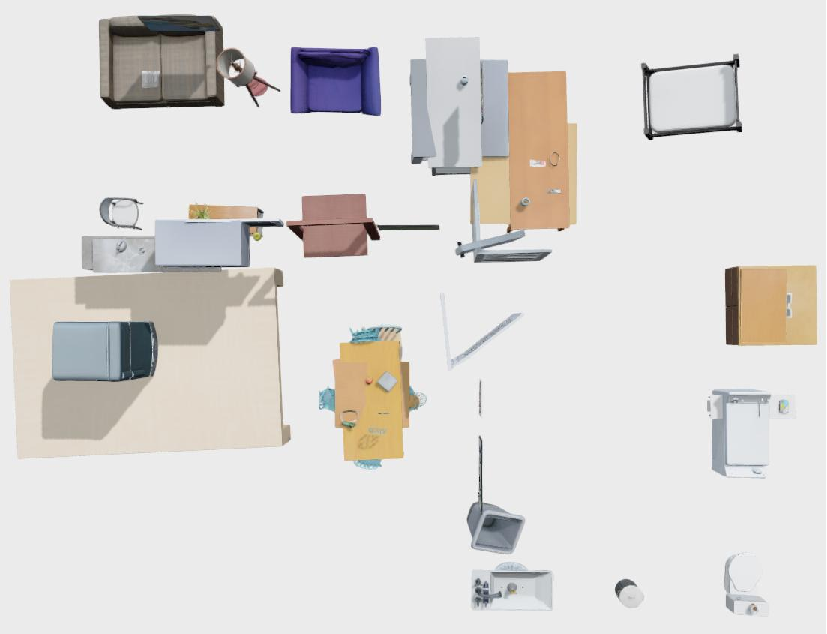
\includegraphics[width=\linewidth]{scene_s200_icp_top.pdf}\caption{asset: YOLOE (ours)}\label{fig:scene_det}
  \end{subfigure}\hfill
  \begin{subfigure}{0.24\textwidth}\centering
    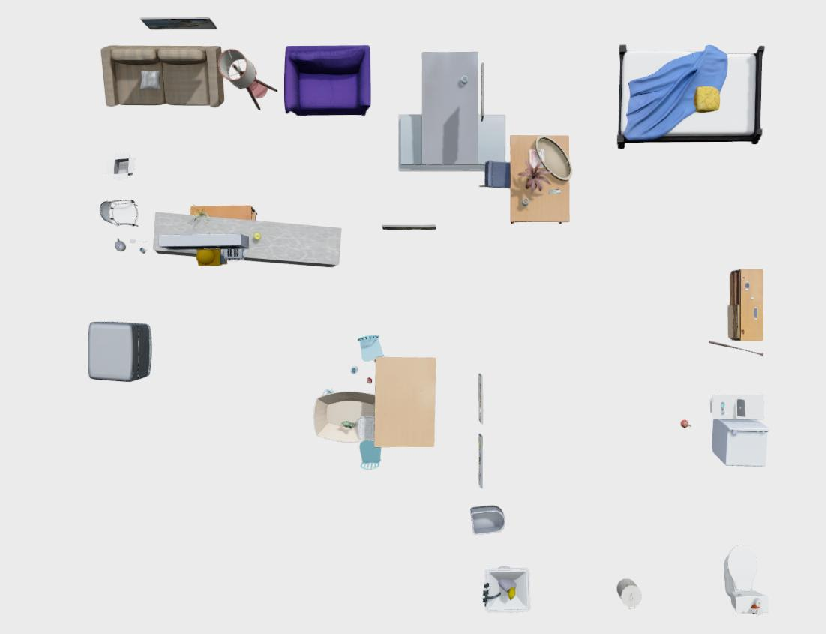
\includegraphics[width=\linewidth]{scene_s200_oracle_scaleicp_top.pdf}\caption{asset: oracle masks}\label{fig:scene_oracle}
  \end{subfigure}
  \caption{\todo{Scene 200, one top-down viewpoint. (a) GT object meshes;
  (b) the clustering-baseline payload --- denoised per-object point clusters
  (noisy, partial); (c) our deployed detector-driven asset map (YOLOE);
  (d) our asset map from oracle GT masks (upper bound). Our node is a clean,
  placed mesh where the clustering line keeps a labelled point cluster; oracle
  masks recover more objects (83 vs 72) --- the perception gap of
  Table~\ref{tab:oracle}.}}
  \label{fig:scenes}
\end{figure*}

\begin{table}[H]
  \centering
  \caption{Perception ceiling (ProcTHOR val-10 means, stride 1, same back-end).
  Two reads: (i) the front-end is the bottleneck --- perfect masks lift IoU-F1
  0.49$\to$0.74 at +ICP; (ii) the registration back-end is needed \emph{even with
  perfect masks} --- oracle placement rises 0.62 (SAM 3D-native) $\to$ 0.74
  (+ICP), and the scale-fit then sharpens size (scale 0.29$\to$0.13).}
  \label{tab:oracle}
  \setlength{\tabcolsep}{4pt}
  \footnotesize
  \begin{tabular}{llccccc}
    \toprule
    masks & reg & IoU-F1 & rec@.5 & S2C & scale\_err & cdF1@1m \\
    \midrule
    YOLOE (ours) & +ICP        & 0.49 & 0.22 & 0.09 & 0.32 & 0.71 \\
    \midrule
    GT (oracle)  & layout      & 0.62 & 0.26 & 0.12 & 0.29 & 0.95 \\
    GT (oracle)  & +ICP        & \textbf{0.74} & 0.33 & 0.14 & 0.32 & \textbf{0.95} \\
    GT (oracle)  & +scale+ICP  & 0.68 & \textbf{0.42} & \textbf{0.33} & \textbf{0.13} & \textbf{0.95} \\
    \bottomrule
  \end{tabular}
\end{table}

\todo{front-end-bottleneck prose (ref Table~\ref{tab:oracle}, Fig~\ref{fig:scenes}) --- build the WEAK->STRONG->PERFECT front-end axis: (1) the front-end is the bottleneck (perfect masks lift IoU-F1 0.49->0.74); (2) the registration back-end is needed even with perfect masks (oracle layout 0.62 -> +icp 0.74), reinforcing C1; (3) BRIDGING SENTENCE (not a parenthetical): even SAM 3, a much stronger open-vocab detector, does not close the gap --- it raises open-set recall but not strict placement (over-detection) and costs ~55x the detector compute, so it is perfect masks, not a bigger detector, that the ceiling needs (App~\ref{app:detector}).}

%==============================================================================
\section{Real-Robot Deployment}
%==============================================================================
% POINTS TO HIT (~1/4 col + fig):
% - Full pipeline runs on a deployed Go2 quadruped and produces an asset-centric
%   USD map consumed by an LLM navigation layer — a qualitative end-to-end
%   demonstration on real hardware.
% - Runtime line: SAM 3D ~24 s/obj + per-stage timing (offline/near-online
%   honesty). \todo: fill per-stage numbers.

\todo{deployment prose + runtime line}

%==============================================================================
\section{Limitations and Conclusion}
%==============================================================================
% POINTS TO HIT (~1/4 col):
% - Placement is observation-limited (registration needs enough views; strict
%   recall floored on partial real depth — shared with baselines).
% - Reprojection scale-fit reads image-plane silhouette spans -> approximate for
%   objects whose axes are rotated off the image plane (front-on assumption).
% - Asset maps approximate surfaces; evaluation is single-session/static.
% - CONCLUSION: the asset-centric node is a usable, simulation-ready alternative
%   to labeled point clusters, and generation demonstrably completes what the
%   robot cannot see.

\todo{limitations + conclusion prose}

%==============================================================================
\appendix
% NOTE: appendices likely count toward the workshop page limit — see the CFP.
% If they do, this is supplementary material / a cut list, not free space.
%==============================================================================

\section{Experimental Configurations}
\label{app:config}
Every comparison is single-variable: the front-end, tracker, depth, and metric
code are held fixed and exactly one factor changes. In simulation
(Table~\ref{tab:sim}) we vary the \emph{node payload and its registration}
across four configurations that share one front-end --- a denoised point cluster
(our clustering baseline, made confound-free), and the SAM 3D asset placed by
SAM 3D's own predicted pose (\texttt{layout}), by our ICP, and by our
scale-fit${+}$ICP. Crucially the three asset configurations reuse a \emph{single}
generation pass: the mesh cache is registration-independent, so each mode is a
re-scoring of the identical meshes rather than a fresh generation, which makes
the placement comparison exact. A companion diagnostic on one scene
(Table~\ref{tab:scale_source}) varies only the \emph{scale source} --- our
RGB-mask reprojection fit versus the extent read from the raw or denoised
depth-cloud bounding box. On hardware we compare against Clio~\cite{clio}, which
we run ourselves and score against the same hand-labelled boxes with the same
metric code (Table~\ref{tab:real}); an internal ablation on our own
pipeline (Table~\ref{tab:real}) then adds
\texttt{layout}$\rightarrow$ICP$\rightarrow$scale-fit$\rightarrow$gate one step
at a time. Because per-scene matched counts on real data are small (1--6), we
additionally report a paired per-object scale test --- objects matched under
both \texttt{layout} and scale-fit, compared by a Wilcoxon signed-rank test ---
that bypasses the matching gate. The shape-completion study
(C2, Fig.~\ref{fig:completion}) places every object by an oracle pose so that
only shape, not placement, is measured.

\section{Metric Definitions}
\label{app:metrics}
Predictions $\{p_i\}$ are matched to ground-truth objects $\{g_j\}$ by Hungarian
assignment maximizing total 3D oriented-box IoU subject to a minimum overlap
$\tau_{\text{IoU}}$; IoU-F1 uses $\tau_{\text{IoU}}=0.25$ and $\text{recall@}0.5$
uses $0.5$.

\paragraph{Pose and size (on matched pairs).}
Centroid error is the median $\lVert c_p-c_g\rVert_2$. A box's principal axes
carry no intrinsic labels, so we resolve the axis correspondence by the
symmetry-aware rotation $g^\star$ that best aligns the predicted frame to ground
truth and measure both orientation and scale under it,
\begin{equation}
  e_{\text{rot}}=\min_{g}\ \angle\!\left(R_p\,g,\,R_g\right),\qquad
  e_{\text{scale}}=\max_{a\in\{1,2,3\}}\left|\frac{\hat{s}_a}{s_a}-1\right| ,
\end{equation}
with $\angle(\cdot,\cdot)$ the geodesic angle and $\hat{s}_a,s_a$ the per-axis
extents under $g^\star$; medians are over matched pairs. \emph{Scan2CAD
accuracy} is the fraction of ground-truth objects with a matched prediction
inside $20\,\text{cm}$, $20^\circ$, and $20\%$ scale simultaneously.

\paragraph{Open-set localization.}
Matching greedily on top-down $(x,y)$ centroid distance within
$\tau=1\,\text{m}$, cd-F1 is the label-agnostic F1 and the class-free recall is
\begin{equation}
  \text{CF-Recall}_{1\text{m}}=\frac{1}{|\{g_j\}|}\sum_j
  \mathbf{1}\!\left[\min_i d_{xy}(p_i,g_j)\le 1\,\text{m}\right],
\end{equation}
the fraction of ground-truth objects with any prediction nearby, independent of
label or box.

\paragraph{Surface reconstruction.}
Pooling all predicted and all ground-truth surface points ($S_P$, $S_G$), the
symmetric scene Chamfer distance is
\begin{equation}
  \text{CD}=\tfrac{1}{2}\!\left[\frac{1}{|S_P|}\!\sum_{x\in S_P}\!\min_{y\in S_G}\!\lVert x-y\rVert
  +\frac{1}{|S_G|}\!\sum_{y\in S_G}\!\min_{x\in S_P}\!\lVert x-y\rVert\right],
\end{equation}
and footprint IoU is the intersection-over-union of occupied $5\,\text{cm}$
ground cells after projecting both clouds to the $(x,y)$ plane. Open-vocabulary
predicted labels are snapped to the nearest scene-vocabulary word by CLIP text
similarity before any label-aware scoring.

\section{Detector Ablation --- Front-End Is Swappable, and Cheap Beats Heavy}
\label{app:detector}
% FRAMING (write prose from these; lead with the COMPUTE TRADEOFF, do NOT
% cherry-pick a single metric — state the recall<->precision trade):
% - The front-end is swappable (infrastructure, Sec.~\ref{sec:frontend}); this is the
%   STRONG middle point of the front-end axis in Sec.~\ref{sec:frontend-bottleneck}
%   (weak YOLOE -> strong SAM 3 -> perfect oracle) --- we test a much stronger
%   open-vocab detector, SAM 3~\cite{sam3}, in YOLOE's place on s200.
% - SAM 3 is concept-prompted: ~1 forward PER vocabulary word per frame (55 for
%   this scene) vs YOLOE's single pass -> O(vocab) compute, tens of minutes/scene
%   vs ~a minute. This is the headline cost.
% - PAYOFF is recall-only: SAM 3 finds/coarsely-places more (best cd-F1 0.82 with
%   the gate) but does NOT improve strict placement (IoU-F1) -- it OVER-DETECTS
%   (116 vs 93 GT), so precision drops (0.62->0.41); the precision gate recovers
%   precision (->0.49) by trading recall.
% - The GT-mask oracle bounds both far above -> the ceiling is perfect masks
%   (precision AND recall), not a bigger detector.
% - CONCLUSION: we default to YOLOE -- near the strict-F1 best at a fraction of
%   the compute; SAM 3 is an offline open-set-recall option, not a live-robot
%   replacement.  (stride-10 caveat: the gate's 6-obs threshold is aggressive on
%   short stride-10 tracks, which is why it also trims YOLOE.)
\begin{table}[H]
  \centering
  \caption{Detector ablation (ProcTHOR s200, stride 10, +ICP; same back-end).
  A heavier open-vocab detector (SAM 3, $\sim$55 concept-forwards/frame vs
  YOLOE's single pass) raises open-set recall (cd-F1, with the gate) but not
  strict placement (IoU-F1): it over-detects, so precision drops; the gate
  trades recall for precision. The GT-mask oracle bounds both. We default to
  the far cheaper YOLOE.}
  \label{tab:detector}
  \setlength{\tabcolsep}{4pt}
  \footnotesize
  \begin{tabular}{lccccc}
    \toprule
    detector & det.\ cost & IoU-F1 & cd-F1 & prec & recall \\
    \midrule
    \textbf{YOLOE (default)}   & $1\times$ & \textbf{0.52} & 0.76 & 0.62 & 0.45 \\
    SAM 3                      & $\sim$55$\times$ & 0.45 & 0.75 & 0.41 & \textbf{0.51} \\
    SAM 3 + gate               & $\sim$55$\times$ & 0.46 & \textbf{0.82} & 0.49 & 0.43 \\
    oracle (GT masks)          & --- & 0.75 & 0.94 & 0.80 & 0.71 \\
    \bottomrule
  \end{tabular}
\end{table}

\todo{detector-ablation prose (ref Table~\ref{tab:detector}) --- lead on the compute tradeoff}

%==============================================================================
\bibliographystyle{IEEEtran}
\bibliography{references}
%==============================================================================

\end{document}
